\section{Introduction \& Background}
In 2018, approximately 261$\si{\tera\watt\hour}$ of power was generated in the Australian electricity sector. Renewables contributed 19\% of the total generation, an increase from 15\% in 2017. The Department of Industry, Science, Energy and Resources have observed an increase in renewable energy generation year-on-year in the electricity generation market since 2008, as shown in Figure \ref{fig:energyts} \cite{Diser2020}.\\

\begin{figure}[ht]
	\centering
	\begin{tikzpicture}
	\begin{axis}[
		no markers,
		tick pos=left,
		width=0.8\textwidth,
		height=0.35\textwidth,
		xlabel=Year,
		x label style={at={(axis description cs:0.5,-0.2)},font=\scriptsize},
		xticklabel style={/pgf/number format/1000 sep=,rotate=60,anchor=east,font=\scriptsize},
		ylabel=Terrawatt hours,
		y label style={font=\scriptsize},
		yticklabel style={/pgf/number format/1000 sep=,font=\scriptsize},
		legend pos={north west},
		legend style={font=\scriptsize}
	]
	\addplot[green!20!gray, ultra thick] table[mark=none, x=year, y=total, col sep=comma] {./figures/101_renewable_energy/renewable_energy.csv};
	\addlegendentry{Total}
	\addplot[green!20!gray, ultra thick, dashed] table[mark=none, x=year, y=renew, col sep=comma] {./figures/101_renewable_energy/renewable_energy.csv};
	\addlegendentry{Renewable}
	\end{axis}
\end{tikzpicture}
	\caption{Power generation from renewable sources (light blue line), and total power generation (dark blue line) in Australia from 1977 to 2018.}
	\label{fig:energyts}
\end{figure}



One of the benefits of transitioning from thermal sources of power generation to renewable sources is reduced greenhouse gas emissions \cite{IPCC2012}; however, this transition is not without its drawbacks. With an increased reliance on renewable power generation sources posing challenges for power system stability owing to load management. A recent example is the system failure in Alice Springs, caused by an event cascade that was triggered by cloud cover shadowing a solar array. The system failure left residents in Alice Springs without power for approximately eight hours \cite{UCNT2019}. An independent investigation highlighted that poor control policies were one of the factors that contributed to the blackout. In this instance, the generator provisioned to ramp up in the event of cloud cover was unable to be controlled. Moreover, generators that were still under the control regime were issued operating set points above their rated capacity, that resulted in thermal overload and subsequent tripping from the protection system \cite{Wilkey2019}.

Current control methods use classical feedback loop techniques. These methods can be brittle when faced with system changes, or scenarios which they were not designed for. An improved controller would be one that can learn and adapt its controller to an unseen system or event, given some broad control objective. This research proposes a deep reinforcement learning (DRL) agent for controlling the frequency of a power system consisting of multiple generators, and multiple load demands with individual stochastic profiles.

\subsection{Power Systems and Frequency}
Interconnected power systems are comprised of power generating units and energy storage systems connected to transmission and distribution networks. Generated power is used to service load demand. A single line diagram of a power network can be seen in Figure \ref{fig:generation}. The diagram shows how thermal generation units (left-hand side), such as coal and nuclear, in addition to renewable sources of generation, like wind and solar provide a power generation mix that is transmitted by a network for the consumers of generated energy: industry and households (right-hand side).
\begin{figure}[ht]
	\centering
	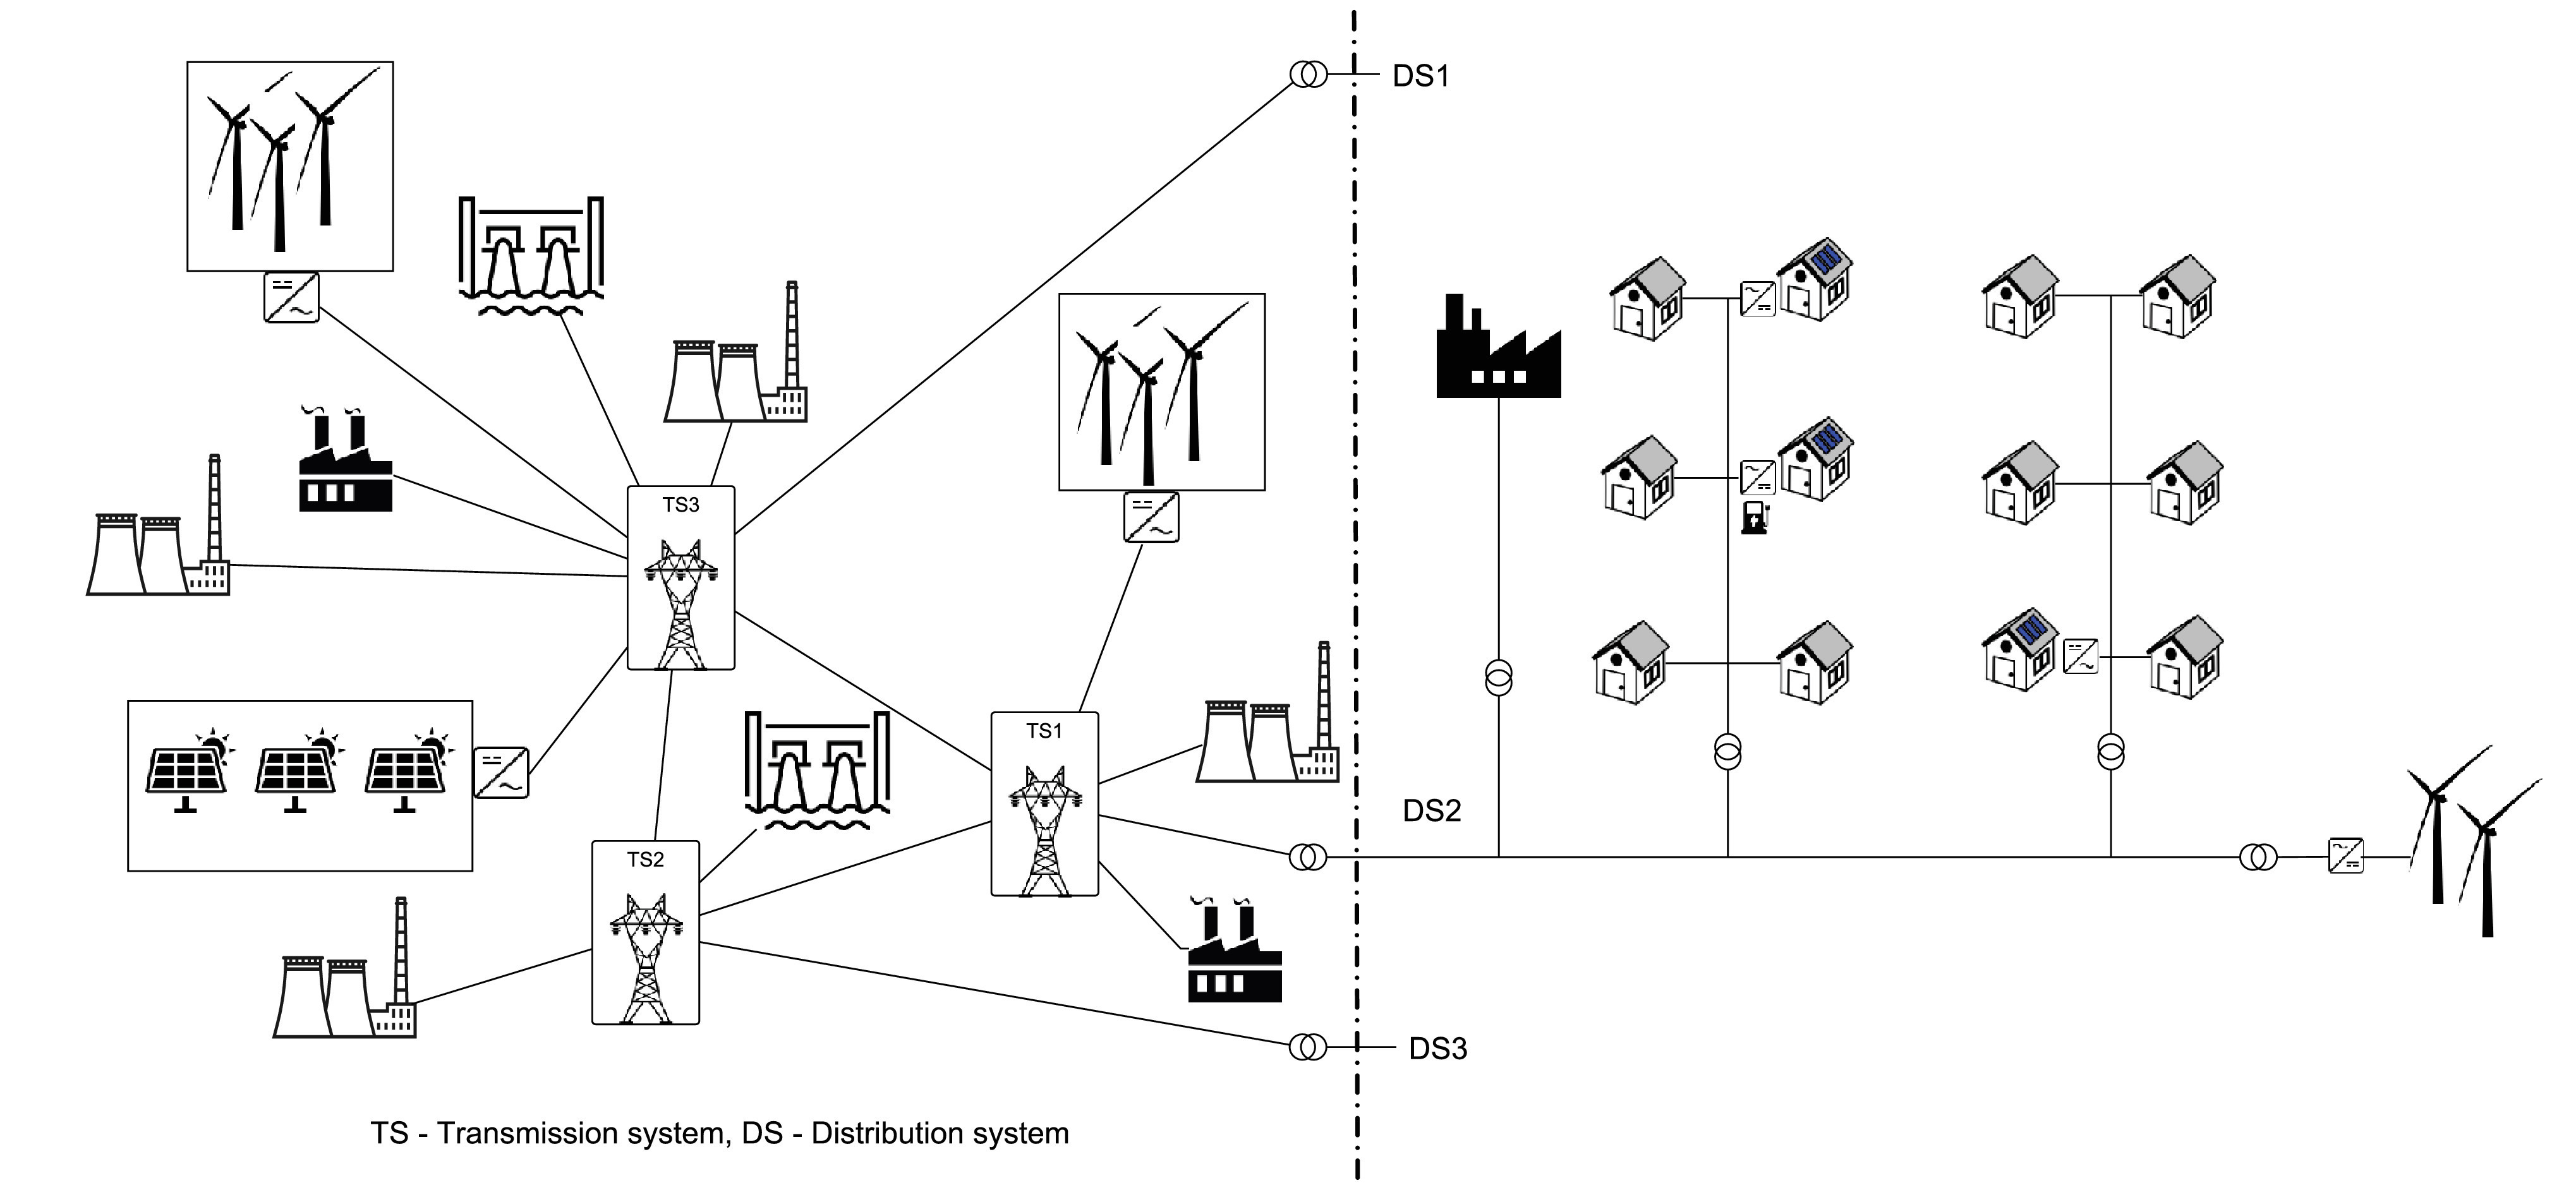
\includegraphics[scale=0.85]{power_system}
	\caption{A single line diagram of a typical power system. The image shows points of generation from thermal and renewable sources, and the subsequent supply of generated energy to meet load demand through the transmission and distribution network \cite{Glavic2019}.}
	\label{fig:generation}
\end{figure}

One of the key elements to successful operation of interconnected power systems is ensuring total load demand is matched with total generation while taking into account power losses involved with generation, transmission, and distribution \cite{Wood2013}. To understand why it is important to match generation with load demand consider the basic operation of a single thermal generator. 
\begin{figure}[h]
	\centering
	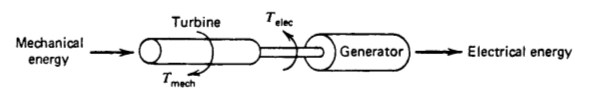
\includegraphics[height=1.4cm]{generation}
	\caption{A thermal generation unit consisting of a prime mover (turbine), and a synchronous machine \cite{Wood2013}.}
	\label{fig:turbine}
\end{figure}

The essential elements of a thermal generator are a prime mover (such as a gas turbine) and a synchronous machine, as depicted in Figure \ref{fig:turbine}. The prime mover provides mechanical torque, $T_{mech}$, which drives the synchronous machine producing electrical energy. In response, the synchronous machine creates an opposing torque that depends on the size of the load demand. This opposing torque is referred to as electrical torque and is denoted as $T_{elec}$. If $\alpha$ represents angular acceleration of the generator rotating mass, and $I$ is its moment of inertia, then by Newton's second law:
\begin{equation}
	T_{mech} - T_{elec} = I \alpha \label{eq:1}
\end{equation}

When $T_{mech}$ equals $T_{elec}$ the system will be in a steady state of zero angular acceleration with a constant angular velocity, $\omega$. Now, if $T_{mech} > T_{elec}$, then the system has an angular acceleration causing the angular velocity, $\omega$, to increase. This results in a frequency increase in the system. Conversely, if $T_{mech} < T_{elec}$ then the angular velocity $\omega$ will decrease, resulting in a frequency decrease. It is important to note that, at any point in time, the total electrical load demand will fluctuate as businesses and households switch grid connected appliances or motors on and off. The result is that an uncontrolled system will have a continually changing frequency. Australia's electricity network is designed to operate at a frequency of 50$\si{\hertz}$. In the majority of network scenarios, the Australian Energy Market Operator (AEMO) has a desired operating range for frequency which lies between 49.85 and 50.15$\si{\hertz}$ \cite{AEMOfreqdev}. Similarly, the Power and Water Corporation (PWC) network technical code for the Northern Territory states that under normal operating conditions frequency should be maintained in the range of 49.80 to 50.20$\si{\hertz}$ \cite{Pwc2013}. Network operation outside of the specified range can cause damage to electrical equipment such as transformers or motors, which are designed to operate at specific frequencies \cite{Sen2014}. Network designers engineer protection schemes so that sustained frequency excursions outside of the allowed range will cause equipment to trip from the network \cite{AEMOpowerfreqriskrev}.

\begin{figure}[ht]
	\centering
	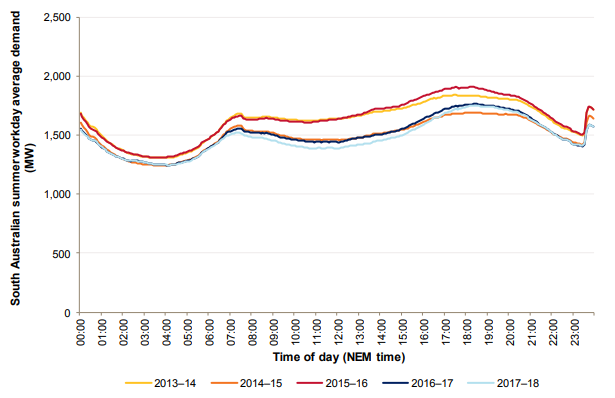
\includegraphics[height=7cm]{load_profile}
	\caption{Weekday energy demand profile in South Australia during summer \cite{Aemosaenergyrep}.}
	\label{fig:energydemand}
\end{figure}

\newpage

Protection schemes tripping equipment from the network is undesirable as this can leave households and industry without power, resulting in economic loss. Further, if disconnections are uncontrolled the system stability is reduced \cite{AEMOpowerfreqriskrev}. System controllers, such as the AEMO and PWC, are interested in being able to control the system to follow changes in load demand so that system frequency is maintained in the allowable range. Additionally, they are interested in control mechanisms to restore frequency excursions as a result of unexpected disturbances. System controllers can use historical data, like that shown in Figure \ref{fig:energydemand}, to forecast daily demand profiles with some reliability. This type of forecasting does not help when trying to predict the occurrence of random disturbances; however, it does provide a starting point for estimating required generation needed to meet demand. It is important to note that forecasting is not perfect. Inevitably mismatches in supply and demand will occur causing small imbalances between $T_{mech}$ and $T_{elec}$, resulting in a change to angular velocity $\omega$ and the network frequency \cite{Glover2012}. To perfectly match supply and demand, system controllers use generators referred to as regulating units, placed under Automatic Generation Control (AGC) \cite{Kothari2011}. A regulating unit is a generator that has the capacity to increase or decrease mechanical torque $T_{mech}$, and AGC is the name used for a system providing control over the mechanical torque output of regulating generators. If the system controller has a sufficient number of regulating units under AGC it can perform two functions: load following, and restoring the system to stable operating conditions in the event of a disturbance \cite{Grainger1994}. Using a regulating unit under AGC control to load follow is referred to, by AEMO, as load following ancillary services \cite{AEMOancilliaryserv}.

\begin{figure}[ht]
\centering
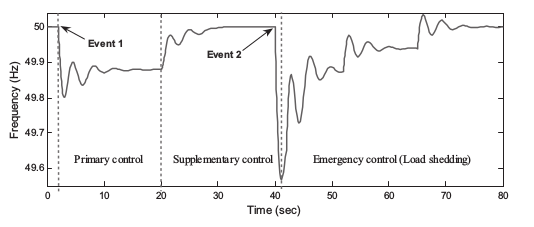
\includegraphics[height=6cm]{frequency_arrest}
\caption{A minor frequency disturbance occurs at the 2 sec mark and primary control systems (governors) arrest the frequency drop. System frequency is adjusted to desired 50$\si{\hertz}$ operating level using AGC control of regulating units. This referred to as supplementary (or secondary) control in the literature. AEMO refers to this as load following ancilliary services. At the 40 sec mark the network experiences a major frequency disturbance which is arrested by emergency control measures such as under-frequency load shedding (UFLS). System restoration is aided using AGC control of regulating units, which AEMO refers to as spinning reserve ancillary services \cite{Bevrani2011}.}
\label{fig:freqarrest}
\end{figure}

\newpage

Load following control adjusts regulating units in order to match supply with a demand load profile, and maintain frequency in a normal operating range a shown in the first 40 seconds of Figure \ref{fig:freqarrest}. Using a regulator under AGC control to restore the system after a major disturbance is referred to, by AEMO, as providing spinning reserve ancillary services. \cite{AEMOancilliaryserv}. When used in either fashion it is important to note that the regulating unit is not responsible for arresting frequency excursions, rather, it is used to restore the system back to the allowable frequency operating range after the frequency excursion has been arrested. An example of a frequency excursion, arrest, and subsequent restoration for minor and major disturbances can be seen in Figure \ref{fig:freqarrest}. AEMO and PWC do not require all generators on the network to act as regulating units since adequate frequency control can be achieved using a subset of the total available generators.


\subsection{Frequency Control for a Single Area System}\label{oneareapowersystem}
The power system model shown in Figure \ref{fig:energyts} depicts total generation coming from many generation assets --- this is complex to model. Researchers often find it useful to divide generation assets into sub-groups referred to as control areas \cite{Kothari2011}. A control area is defined as a subset of generators that are in close proximity to each other and constitute a coherent group that speed up and slow down together, maintaining their relative power angles \cite{Kothari2011}. Therefore, the total network is comprised of many interconnected control areas. An example of this can be seen in Figure \ref{fig:interconnectedpa}. Notice that for each area there is only one load and one generator.
\begin{figure}[ht]
	\centering
	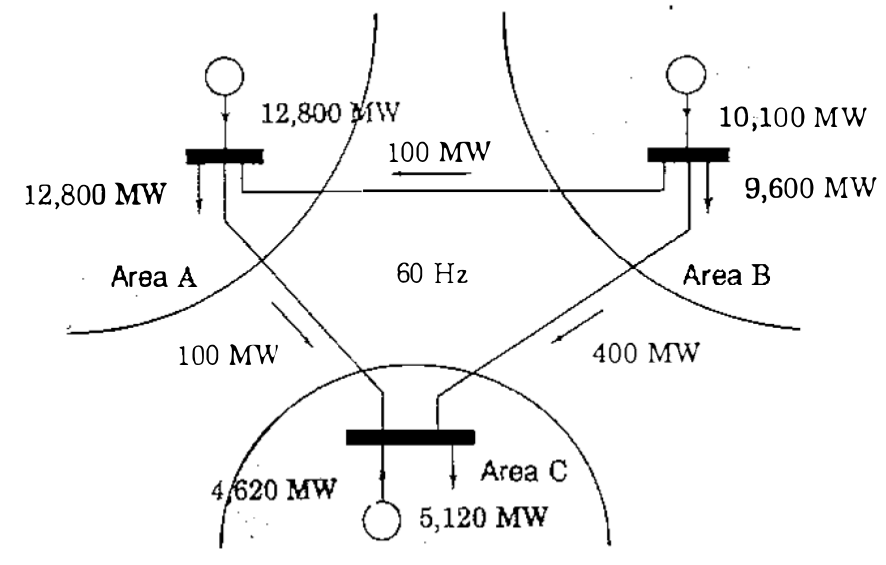
\includegraphics[height=8cm]{multiple_area_system}
	\caption{An example of three interconnected control areas in a 60$\si{\hertz}$ power system. The interconnections allow power to flow from one area to another, allowing generators to service loads from different areas. Each control area consists of several generators and loads, but are modelled with a single generator and single load for simplicity \cite{Grainger1994}.}
	\label{fig:interconnectedpa}
\end{figure}

Typically, for each control area, researchers will aggregate many loads into a single load, and many generators into a single generator. This simplifies the model further \cite{Grainger1994}. The simplest power system to control is one that consists of a single control area. A single control area power system has no interconnections to any other control area. It is comprised of a consumer load demand, and a set of generators, some of which are acting as regulating units. As previously mentioned, for modelling simplicity, loads are aggregated to a single load, and generators can be aggregated to a single generator. This simple system is well understood. It is generally acknowledged that a speed droop governor feedback control regime will perform primary frequency control, and an AGC feedback loop is used to perform secondary frequency control when restoring a minor frequency excursion \cite{Wood2013, Grainger1994, Kothari2011, Kundur1994}. A particularly well laid out approach to developing linear models for the turbine, generator, load, and governor was presented by Kundur \cite{Kundur1994}. The full model is shown in Figure \ref{fig:singleareacontrol}. This particular model provides generator models for regulating and non-regulating generators. The governor blocks are first-order linear models of the speed governors. The turbine blocks are first-order models of the turbines. The final block is the generator load, which is also a first order system. The AGC feedback loop uses an integral controller.

\begin{figure}[ht]
\centering
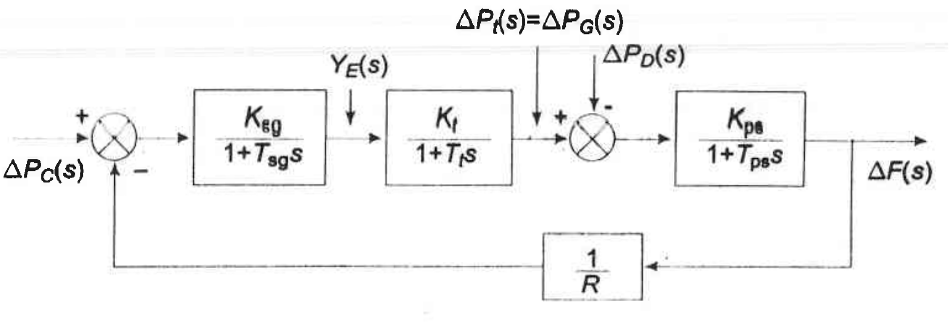
\includegraphics[height=8cm]{single_area_control}
\caption{A classical feedback control approach for a single control area power system. The system is comprised of a first order models for both turbines, and generators. The governor controllers are also first order models. AGC is implemented using an integral control block in a feedback loop \cite{Kundur1994}.}
\label{fig:singleareacontrol}
\end{figure}

\newpage

\subsection{Frequency Control for Two Area System}
The single area system presented in Section \ref{oneareapowersystem} is useful to help understand the role of governors and AGC in controlling power system frequency. In reality, power systems are comprised of many control areas connected by transmission lines (referred to in the literature as tie lines). Often it is the case that there is some net power transfer over the tie lines, enforceable by economic contract. Single area models do not provide for this additional complexity.

\begin{figure}[ht]
	\centering
	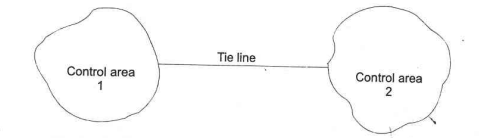
\includegraphics[height=3cm]{two_area_system}
	\caption{A two area power system comprised of generators and load connected via a tie line. Power flows from one area to the other depending on the power demands.}
	\label{fig:twoareapower}
\end{figure}

Distinct control areas are typically thought of as different participants in the generation market, or simply as different regions in which generation assets are based \cite{Kothari2011}.

\begin{figure}[ht]
	\centering
	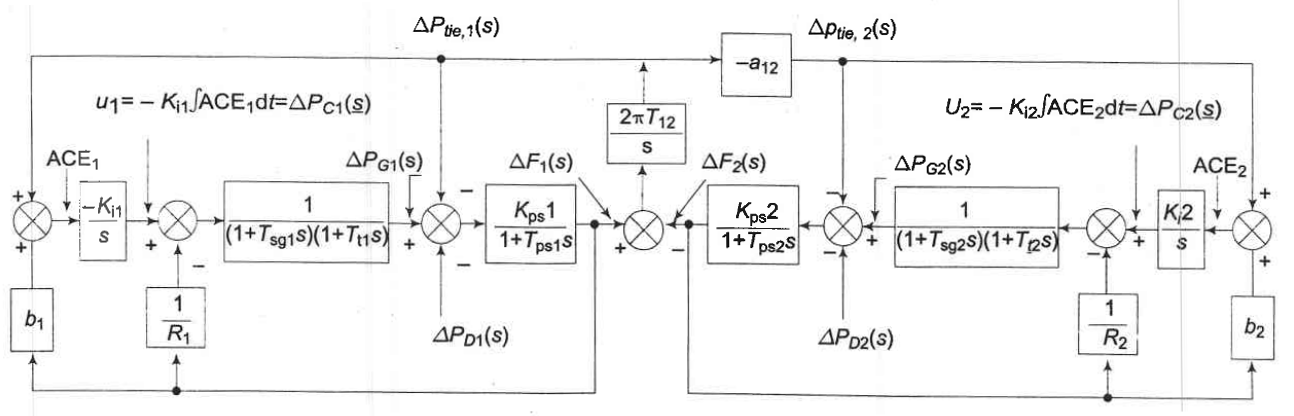
\includegraphics[height=12cm]{two_area_control_block}
	\caption{A classical feedback control approach to a two area power system \cite{Kundur1994}.}
	\label{fig:twoareacontrolblock}
\end{figure}

The simplest model that includes tie lines is the two area power system, shown in Figure \ref{fig:twoareapower}. The control objective with this system is to maintain the inter-area power transfer, whilst regulating the frequency of each area. An AGC integral feedback loop on regulating units, like that shown in Figure \ref{fig:singleareacontrol}, would ensure that power system frequency is maintained, however, would not guarantee inter-area power transfer agreements are observed. Violation of power transfer contracts due to control issues does not allow for a stable market in which energy can be reliably traded. Fortunately, multi control area power systems are well understood. Linear models have been developed to simulate these systems, and classical control approaches have been successfully implemented to meet the new control objectives. In order to achieve this, a metric called Area Control Error (ACE) is used in the AGC feedback loop for each control area. ACE is a linear combination of the frequency deviations and the . The implementation of this control system is shown in Figure \ref{fig:twoareacontrolblock}.


\subsection{Reinforcement Learning}
Reinforcement Learning (RL) is a branch of machine learning that is concerned with how agents make sequential decisions to maximise some notion of a cumulative reward. It is a simple idea that allowed Google's DRL agent, AlphaGo, to beat the world's best players in a game of Go \cite{Silver2016}. One of the important aspects of RL is the underlying architecture of the model, which allows for generalisation to many different applications, albeit the models do require training with different data sets for each application. A brief overview of key architectural components of RL can be found in \S{}\S{}\ref{mdp1} and \ref{mdp2}. \S{}\ref{rl} gives details on how these components are implemented to build an agent that can perform a control activity for some application.

\subsubsection{Markov Decision Process}\label{mdp1}
Suppose an agent exists in some environment that is comprised of many discrete states, $s \in S$, such that $S$ denotes the state space. At any discrete point in time the agent can take an action $a \in A$, where $A$ denotes the action space. When the agent takes an action in a given state, the agent receives some reward, denoted with $r \in R$, where $R$ is the reward set. If an agent is in a given state, $s$, and takes and action, $a$, this will transition the agent to a new state, $s'$, and yield reward, $r$, with some given probability --- these are referred to as state transition probabilities. Transition probabilities are denoted as follows:
\begin{equation}
P(S_{t+1}=s', R_{t+1}=r \ | \ S_t = s, A_t = a)\label{eq:2}
\end{equation}

The set of parameters outlined above, and equation \ref{eq:2}, make up a framework referred to as a Markov Decision Process (MDP) \cite{Bellm1957}. The MDP framework is important to understanding how RL works; however, it must be noted that it is not necessary for the agent to have any information about the state transition dynamics to develop an effective control regime.

\subsubsection{Return, Episodes, and Policy}\label{mdp2}
As the agent takes actions at each discrete time step, it receives a reward. The cumulative sum of this reward is referred to as the return \cite{openai2018}. For $N$ discrete time steps the return is denoted as:
\begin{equation}
G_t = r_t + r_{1+1} + r_{t+2} + \ldots + r_{N-1}\label{eq:3}
\end{equation}

Often it is convenient to make future rewards less important than more immediate rewards. This is achieved by multiplying each reward in the sequence by a discount factor, $\gamma \in [0,1]$. Equation \ref{eq:3} then becomes:
\begin{equation}
G_t = r_t + \gamma \ r_{1+1} + \gamma\mystrut^2 r_{t+2} + \ldots + \gamma\mystrut^{N-1} r_{N-1} = \sum_{k = 0}^{N-1} \gamma\mystrut^k r_{t+k}
\end{equation}

The duration of time that an agent will cumulate reward is referred to as an episode. An episode is made up of a beginning, a middle, and an end. Typically, this consists of an RL agent beginning in some initial state. As time passes the agent takes actions, undergoes state transitions, and collects rewards. The episode concludes when the agent reaches a terminal state. At the episode conclusion, the agent receives it's cumulative reward \cite{Kaelbling1996}.

Finally, in order for the robot to act within the environment, it needs to have a policy. A policy, $\pi$, is defined as a mapping from states to actions, i.e. a rule which determines what action the robot will take for a given state. A deterministic policy, $\pi (s)$, maps a single action to a single state. A stochastic policy, $\pi (a | s)$, defines a probability distribution over the actions for a given state. An optimal policy, denoted $\pi^*$, is a policy which will maximise the cumulative reward that the agent receives over an episode \cite{Bellm1954}. It can be thought of as the best control policy an agent can have for the given the environment and cumulative reward function.

\subsubsection{How Does an RL Agent Learn?}\label{rl}
The main objective of RL is to develop an optimal policy. There are many algorithmic approaches to building an optimal policy. One of the most common implementations is called Q-learning. This approach focuses on finding q-values for each state-action pair. A q-value can be thought of as an ordinal value that is discovered and assigned to a state-action pair that tells the agent how important an action is relative to the rest of the actions in a given state. The agent normally starts with a randomised policy meaning that all the q-values are set to zero. This will lead the agent to take actions at random and explore the state-action space. Higher q-values are then assigned to state-action pairs that the agent classifies as useful for building a high cumulative reward. Similarly, the agent assigns low q-values to state-action pairs that do not lead to high cumulative rewards. This process is akin to the agent modifying its policy. The q-value modification process is iterated over many episodes and eventually the agent policy converges on an optimal policy. Often the q-values are presented in a tabular format that the literature refers to as a Q-table. An example of a Q-table can be seen in Figure \ref{fig:qtable}. Rows represent different states, and columns represent different actions. Values in each cell provide an ordinance on how valuable each action is for a given state. The agent only needs to understand inputs that uniquely define a state, and the actions it can take in order to learn an optimal policy. It is not necessary for the agent to know the state transition dynamics of the system, described by Equation \ref{eq:2}. Therefore, an agent can learn to control a system for which is does not have a mathematical model.
\begin{figure}[ht]
	\centering
	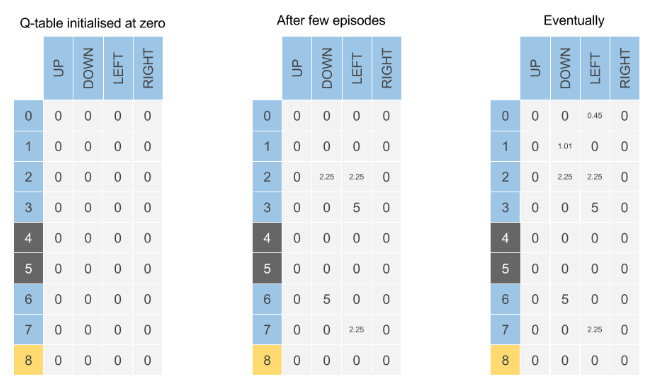
\includegraphics[height=8cm]{q_table}
	\caption{The Q-table on the left shows the initialised policy when the agent begins learning. The middle and rightmost Q-tables show the agent developing an understanding of which actions are valuable in which states.(REFERENCE)}
	\label{fig:qtable}
\end{figure}

\subsection{Deep Reinforcement Learning}
For low dimensional state-action spaces RL leads to policy convergence in a reasonable time frame. As state-action space dimensionality increases Q-Learning models experience difficulty. Owing to increasing computing demands, it becomes difficult for the discrete RL algorithm to visit every state-action pair unless the computational power is dramatically increased. The impace of dimensionality on Q-learning has been previously reported (REFERENCES). Stopping policy discovery prior to optimal policy convergence is not an option under problems with high dimensionality as this results in sparse Q-tables (mostly populated with zeros).
\begin{figure}[ht]
\centering
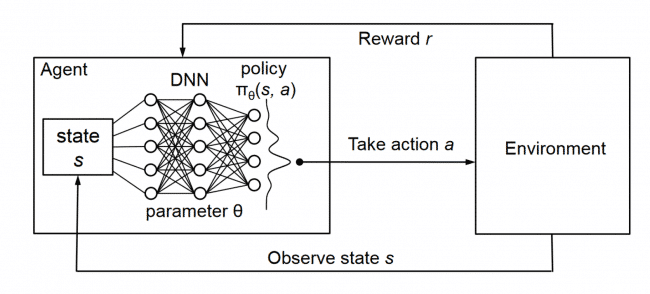
\includegraphics[height=5cm]{deep_reinforcement_learning}
\caption{The agent interacts with the environment by taking actions, which affect the state it is in and the reward it receives. The rewards allow agent to adjust the weights in the neural net to build better policies.}
\end{figure}

The interpretation of sparseness in Q-tables is that the agent does not have a complete knowledge of optimal actions for every given state. This leads to sub-optimal policies. In order to improve policy, for RL problems with high dimensional state spaces, the discrete Q-table is replaced with a function approximator known as a neural network. A high level overview of the architecture can be seen in Figure 11. It is the neural network architecture in which the agent's policy is implemented. The agent learns by adjusting weights in the neural network to change the policy. This approach is significant because neural networks are good at generalising, and hence the agent does not need to visit every state action pair to be able to make good decisions.